% Credits are indicated where needed. The general idea is based on a template by Vel (vel@LaTeXTemplates.com) and Frits Wenneker.

\documentclass[11pt, a4paper]{article} % General settings in the beginning (defines the document class of your paper)
% 11pt = is the font size
% A4 is the paper size
% “article” is your document class

%----------------------------------------------------------------------------------------
%	Packages
%----------------------------------------------------------------------------------------

% Necessary
\usepackage[german,english]{babel} % English and German language 
\usepackage{booktabs} % Horizontal rules in tables 
% For generating tables, use “LaTeX” online generator (https://www.tablesgenerator.com)
\usepackage{comment} % Necessary to comment several paragraphs at once
\usepackage[utf8]{inputenc} % Required for international characters
\usepackage[T1]{fontenc} % Required for output font encoding for international characters

% Might be helpful
\usepackage{amsmath,amsfonts,amsthm} % Math packages which might be useful for equations
\usepackage{tikz} % For tikz figures (to draw arrow diagrams, see a guide how to use them)
\usepackage{tikz-cd}
\usetikzlibrary{positioning,arrows} % Adding libraries for arrows
\usetikzlibrary{decorations.pathreplacing} % Adding libraries for decorations and paths
\usepackage{tikzsymbols} % For amazing symbols ;) https://mirror.hmc.edu/ctan/graphics/pgf/contrib/tikzsymbols/tikzsymbols.pdf 
\usepackage{blindtext} % To add some blind text in your paper


%---------------------------------------------------------------------------------
% Additional settings
%---------------------------------------------------------------------------------

%---------------------------------------------------------------------------------
% Define your margins
\usepackage{geometry} % Necessary package for defining margins

\geometry{
	top=2cm, % Defines top margin
	bottom=2cm, % Defines bottom margin
	left=2.2cm, % Defines left margin
	right=2.2cm, % Defines right margin
	includehead, % Includes space for a header
	%includefoot, % Includes space for a footer
	%showframe, % Uncomment if you want to show how it looks on the page 
}

\setlength{\parindent}{15pt} % Adjust to set you indent globally 

%---------------------------------------------------------------------------------
% Define your spacing
\usepackage{setspace} % Required for spacing
% Two options:
\linespread{1.5}
%\onehalfspacing % one-half-spacing linespread

%----------------------------------------------------------------------------------------
% Define your fonts
\usepackage[T1]{fontenc} % Output font encoding for international characters
\usepackage[utf8]{inputenc} % Required for inputting international characters

\usepackage{XCharter} % Use the XCharter font


%---------------------------------------------------------------------------------
% Define your headers and footers

\usepackage{fancyhdr} % Package is needed to define header and footer
\pagestyle{fancy} % Allows you to customize the headers and footers

%\renewcommand{\sectionmark}[1]{\markboth{#1}{}} % Removes the section number from the header when \leftmark is used

% Headers
\lhead{STAT 333} % Define left header
\chead{\textit{}} % Define center header - e.g. add your paper title
\rhead{Regression Runner} % Define right header

% Footers
\lfoot{} % Define left footer
\cfoot{\footnotesize \thepage} % Define center footer
\rfoot{ } % Define right footer

%---------------------------------------------------------------------------------
%	Add information on bibliography
\usepackage{natbib} % Use natbib for citing
\usepackage{har2nat} % Allows to use harvard package with natbib https://mirror.reismil.ch/CTAN/macros/latex/contrib/har2nat/har2nat.pdf

% For citing with natbib, you may want to use this reference sheet: 
% http://merkel.texture.rocks/Latex/natbib.php

%---------------------------------------------------------------------------------
% Add field for signature (Reference: https://tex.stackexchange.com/questions/35942/how-to-create-a-signature-date-page)
\newcommand{\signature}[2][5cm]{%
  \begin{tabular}{@{}p{#1}@{}}
    #2 \\[2\normalbaselineskip] \hrule \\[0pt]
    {\small \textit{Signature}} \\[2\normalbaselineskip] \hrule \\[0pt]
    {\small \textit{Place, Date}}
  \end{tabular}
}
%---------------------------------------------------------------------------------
%	General information
%---------------------------------------------------------------------------------
\title{title} % Adds your title
\author{
Stanley Zheng \space Eric \space Lucas
% Add your first and last name
    \thanks{Equal contribution} % Adds a footnote to your title
    %\institution{YOUR INSTITUTION} % Adds your institution
  }

\date{\small \today} % Adds the current date to your “cover” page; leave empty if you do not want to add a date


%---------------------------------------------------------------------------------
%	Define what’s in your document
%---------------------------------------------------------------------------------

\begin{document}


% If you want a cover page, uncomment "%---------------------------------------------------------------------------------
% Cover page
%---------------------------------------------------------------------------------

% Here are more templates for other cover pages: https://www.latextemplates.com/cat/title-pages

% This example is based on this cover page example: https://www.latextemplates.com/template/academic-title-page

\begin{titlepage} % Starts new environment where the page number is not displayed and the count starts at 1 for the next page

%------------------------------------------------
%	Institutional information
%------------------------------------------------
	
\begin{minipage}{0.4\textwidth} % Begins new environment (like a text box)
    \begin{flushleft} % Sets environment on the left side of the paper
    \large
    University of XX\\ % Add your institution
    Chair of Political Science IV\\ % Add the chair
    Fall 2018\\ % Add term
    COURSE TITLE\\ % Add course title
    Supervisor: NAME % Add instructor/supervisor name 
    \end{flushleft}
\end{minipage}
	
\vspace*{2in} % Adds some space in-between
	
\center % Centre everything on the page

%------------------------------------------------
%	Main part
%------------------------------------------------
	
{\huge\bfseries 值jij}\\[0.4cm] % Add your paper title 
{\large\today}\\[0.4cm] % Add date (current day)
FIRSTNAME LASTNAME % Add your name
	
\vfill % Adds additional space

%------------------------------------------------
%	General information about the author
%------------------------------------------------

\vfill % Adds additional space

Your contact info \\ % Add your contact info
Your Program \\ % Add info about your program
Semester you are enrolled \\ % Add info about your semester

\vfill % Adds additional space

%------------------------------------------------
%	Word count
%------------------------------------------------

\vfill % Adds additional space
	
Word count: XXXX % To indicate the word count
% How to check words in a LaTeX document: https://www.overleaf.com/help/85-is-there-a-way-to-run-a-word-count-that-doesnt-include-latex-commands
	

	
\end{titlepage}" and uncomment "\begin{comment}" and "\end{comment}" to comment the following lines
%%---------------------------------------------------------------------------------
% Cover page
%---------------------------------------------------------------------------------

% Here are more templates for other cover pages: https://www.latextemplates.com/cat/title-pages

% This example is based on this cover page example: https://www.latextemplates.com/template/academic-title-page

\begin{titlepage} % Starts new environment where the page number is not displayed and the count starts at 1 for the next page

%------------------------------------------------
%	Institutional information
%------------------------------------------------
	
\begin{minipage}{0.4\textwidth} % Begins new environment (like a text box)
    \begin{flushleft} % Sets environment on the left side of the paper
    \large
    University of XX\\ % Add your institution
    Chair of Political Science IV\\ % Add the chair
    Fall 2018\\ % Add term
    COURSE TITLE\\ % Add course title
    Supervisor: NAME % Add instructor/supervisor name 
    \end{flushleft}
\end{minipage}
	
\vspace*{2in} % Adds some space in-between
	
\center % Centre everything on the page

%------------------------------------------------
%	Main part
%------------------------------------------------
	
{\huge\bfseries 值jij}\\[0.4cm] % Add your paper title 
{\large\today}\\[0.4cm] % Add date (current day)
FIRSTNAME LASTNAME % Add your name
	
\vfill % Adds additional space

%------------------------------------------------
%	General information about the author
%------------------------------------------------

\vfill % Adds additional space

Your contact info \\ % Add your contact info
Your Program \\ % Add info about your program
Semester you are enrolled \\ % Add info about your semester

\vfill % Adds additional space

%------------------------------------------------
%	Word count
%------------------------------------------------

\vfill % Adds additional space
	
Word count: XXXX % To indicate the word count
% How to check words in a LaTeX document: https://www.overleaf.com/help/85-is-there-a-way-to-run-a-word-count-that-doesnt-include-latex-commands
	

	
\end{titlepage}

%\begin{comment}
\maketitle % Print your title, author name and date; comment if you want a cover page 

% \begin{center} % Center text
%     Word count: XXXX
% % How to check words in a LaTeX document: https://www.overleaf.com/help/85-is-there-a-way-to-run-a-word-count-that-doesnt-include-latex-commands
% \end{center}
%\end{comment}

%----------------------------------------------------------------------------------------
% Abstract
%----------------------------------------------------------------------------------------
\setcounter{page}{1} % Sets counter of page to 1
\section{Abstract} % Adds a section title
This project investigates how the relationship between three-point shooting and team success 
in the NBA has evolved over the past two decades. Using team-level data from the 2003-04 and 
2023-24 regular seasons obtained via the NBA API, we construct multiple linear regression 
models to examine the effects of three-point percentage (3P\%), two-point percentage (2P\%), 
and shot selection proportions on win rate. Our analysis reveals a statistically significant 
interaction between 3P\% and era, indicating that the marginal impact of three-point accuracy 
on team success has increased substantially in the modern NBA. While 3P\% showed no significant 
association with win rate in 2003-04, it has become a strong predictor in 2023-24—even after 
controlling for other efficiency metrics. This shift reflects a broader structural change in 
league strategy, marking the emergence of a “three-point era.” Though based on observational 
data, the use of interaction terms allows for a quasi-causal interpretation of this evolving 
relationship.
%----------------------------------------------------------------------------------------
% Introduction
%----------------------------------------------------------------------------------------
\section{Introduction} % Add a section title
\subsection{Motivation} % Add a subsection title
Over the past two decades, the NBA has undergone a dramatic transformation in offensive strategy. 
The rise of “small-ball” systems and analytics-driven decision making has led to a surge in 
three-point attempts, reshaping how teams space the floor, select shots, and build rosters. 
Players like Stephen Curry have redefined the value of long-range shooting, prompting coaches 
and front offices to reconsider the role of the three-point shot in winning games. This project 
is motivated by a key question at the heart of this shift: Has the importance of three-point 
shooting truly increased over time, and if so, how does it compare to traditional metrics like 
two-point efficiency or shot selection proportions? By using regression analysis on team-level 
data from different seansons, we aim to quantify how the statistical relationship 
between shooting performance and win rate has changed. In the era of big data, we believe that 
understanding these evolving dynamics can help teams identify actionable areas for improvement 
and optimize offensive strategies for greater success.
\subsection{Dataset}
Our dataset is sourced from the NBA's public API, an online interface that provides comprehensive 
and standardized statistics for teams and players across multiple seasons. The NBA API offers detailed 
data covering a wide range of performance categories, including shooting statistics, rebounding, passing, 
turnovers, fouls, player efficiency metrics, and advanced team analytics.

The full dataset records team-level aggregates for each regular season, capturing key indicators such as 
field goal percentages, three-point and two-point shooting volume and accuracy, free throw statistics, 
rebound counts, assist counts, turnover rates, steal and block numbers, and overall team performance metrics 
like win-loss records and plus-minus ratings. The structure of the dataset is shown in the Figure \ref{fig:original_data}, and the 
detailed explanation of each variable is shown in the Appendix.
\begin{figure}[htbp]
    \centering
    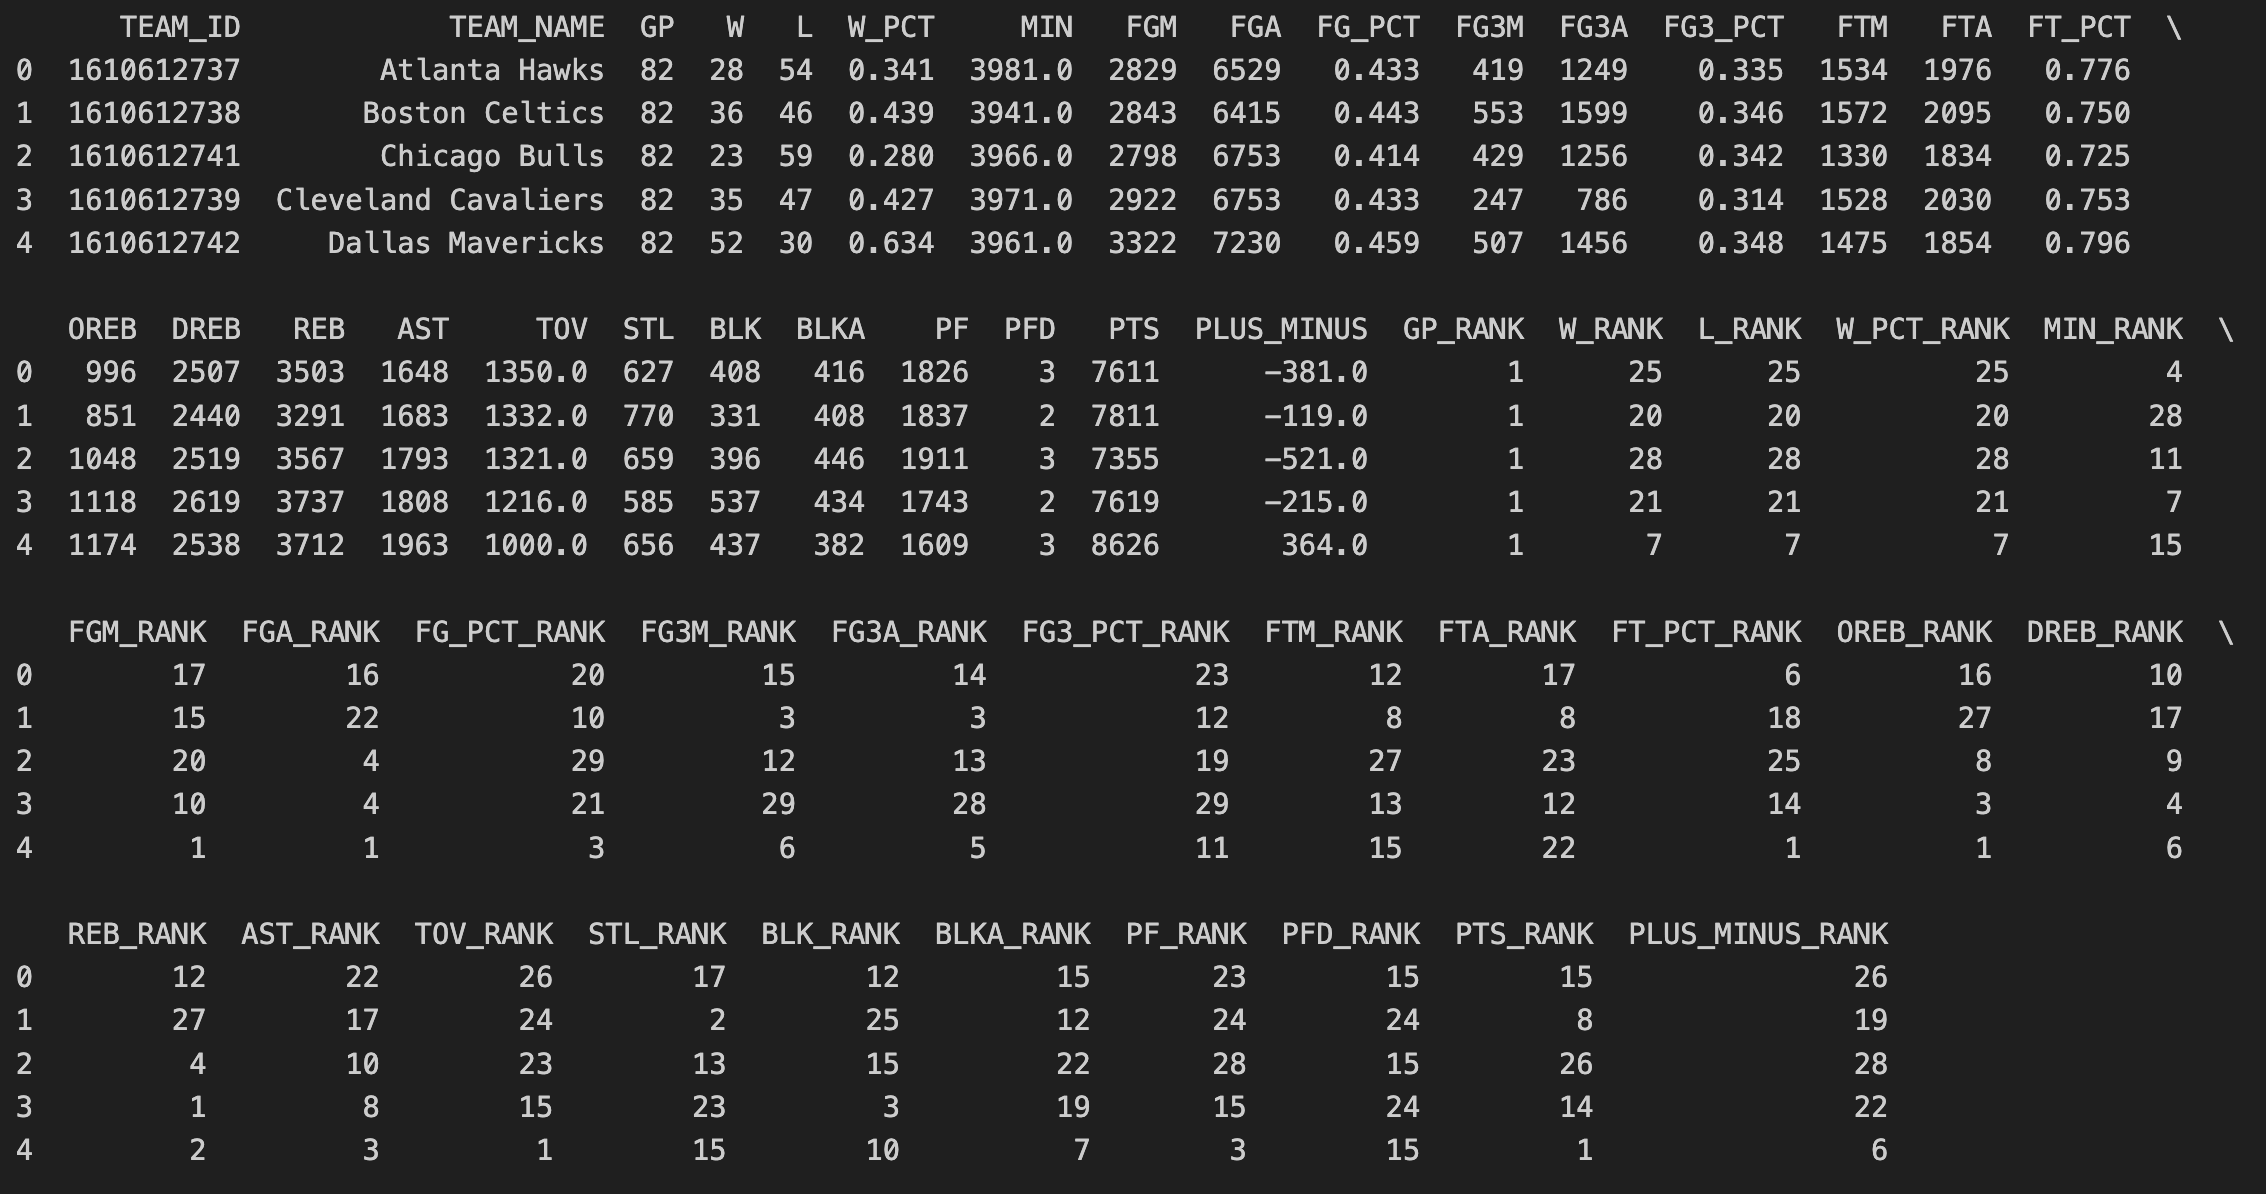
\includegraphics[width=0.9\textwidth]{figure/original_data.png}
    \caption{The Description of The Original Dataset.}
    \label{fig:original_data}
\end{figure}

For our analysis, we primarily focus on shooting-related metrics, including three-point field goal percentage (3P\%), 
two-point field goal percentage (2P\%), three-point attempt rate (3PA rate), and two-point attempt rate (2PA rate). 
Three-point and two-point attempt rates are computed as the proportion of total field goal attempts originating from 
each respective shot zone. To control for other aspects of team strength that may confound the relationship between 
shooting performance and win rate, we also incorporate variables such as total rebounds, turnovers, and other 
team-level performance indicators as covariates in our regression models. This approach allows us to better isolate 
the specific impact of shooting metrics on team success across different eras.
% Some example text
% \LaTeX allows you to highlight text in various ways: \textbf{bold}, \textit{italics}, with \textsc{small caps} or \texttt{as a coding font}.\footnote{ This command adds a footnote to your text.} 
% Citing in \LaTeX is easy. You could easier cite with the text flow like this ``Referring to \citet{collier2004greed} ...''  or at the end of the sentence \cite{collier2004greed}. You can also cite pages like this \citep[55]{collier2004greed}. If you want to add an additional note, you might want to do it this way \citep[cp.][22]{collier2004greed} or like this \citep[cp.][]{collier2004greed}.\\

%----------------------------------------------------------------------------------------
% Data Analysis
%----------------------------------------------------------------------------------------

\section{Data Analysis}
\subsection{Data Preprocess}
Our data preprocessing involved three major steps. First, we retrieved the raw data from an API, where each table corresponds 
to a different season, and each row records a team's performance for that year. Therefore, our unit of analysis is team/year.

As shown in Figure \ref{fig:original_data}, a large portion of the raw variables consisted of rankings (e.g., team rank in various metrics), 
which we decided to remove, as they are not suitable for our analysis. We also observed that the raw data already included some 
basic performance statistics, such as win percentage (W\_PCT) and three-point shooting percentage(FG3\_PCT). However, since the available 
statistics were limited to only a few dimensions, we manually calculated additional variables: win rate(WinRate), three-point attempt rate(3P\_ratio), 
three-point shooting percentage(3P\%), and two-point shooting percentage(2P\%).

We found that the three-point attempt rate and the two-point attempt rate are in a perfect linear relationship (they add up to 1), 
so we included only the three-point attempt rate in our models to avoid multicollinearity.

Finally, because most of our key variables, such as win rate and shooting percentages, naturally fall within the range [0, 1], 
we applied normalization to the other numerical variables as well to ensure these variables also fall with in the range [0, 1], 
which maintains the consistency across features. 

\subsection{Data Visulization}
To motivate our investigation into the evolving impact of three-point shooting on team success, we first examine two sets of histograms 
comparing the 2005-2009 and 2020-2024 NBA regular seasons.

The first set of histograms(Figure \ref{fig:3P_shooting_percent}) shows the three-point shooting percentage (3P\%), capturing efficiency on three-point attempts. While the 
distributions for the two periods overlap significantly, there is a modest rightward shift, indicating that teams have become slightly 
more accurate from beyond the arc over time. This suggests that the increase in three-point volume has not come at the expense of efficiency, 
but rather, teams have adapted by developing better shooters and improving shot quality.

\begin{figure}[htbp]
    \centering
    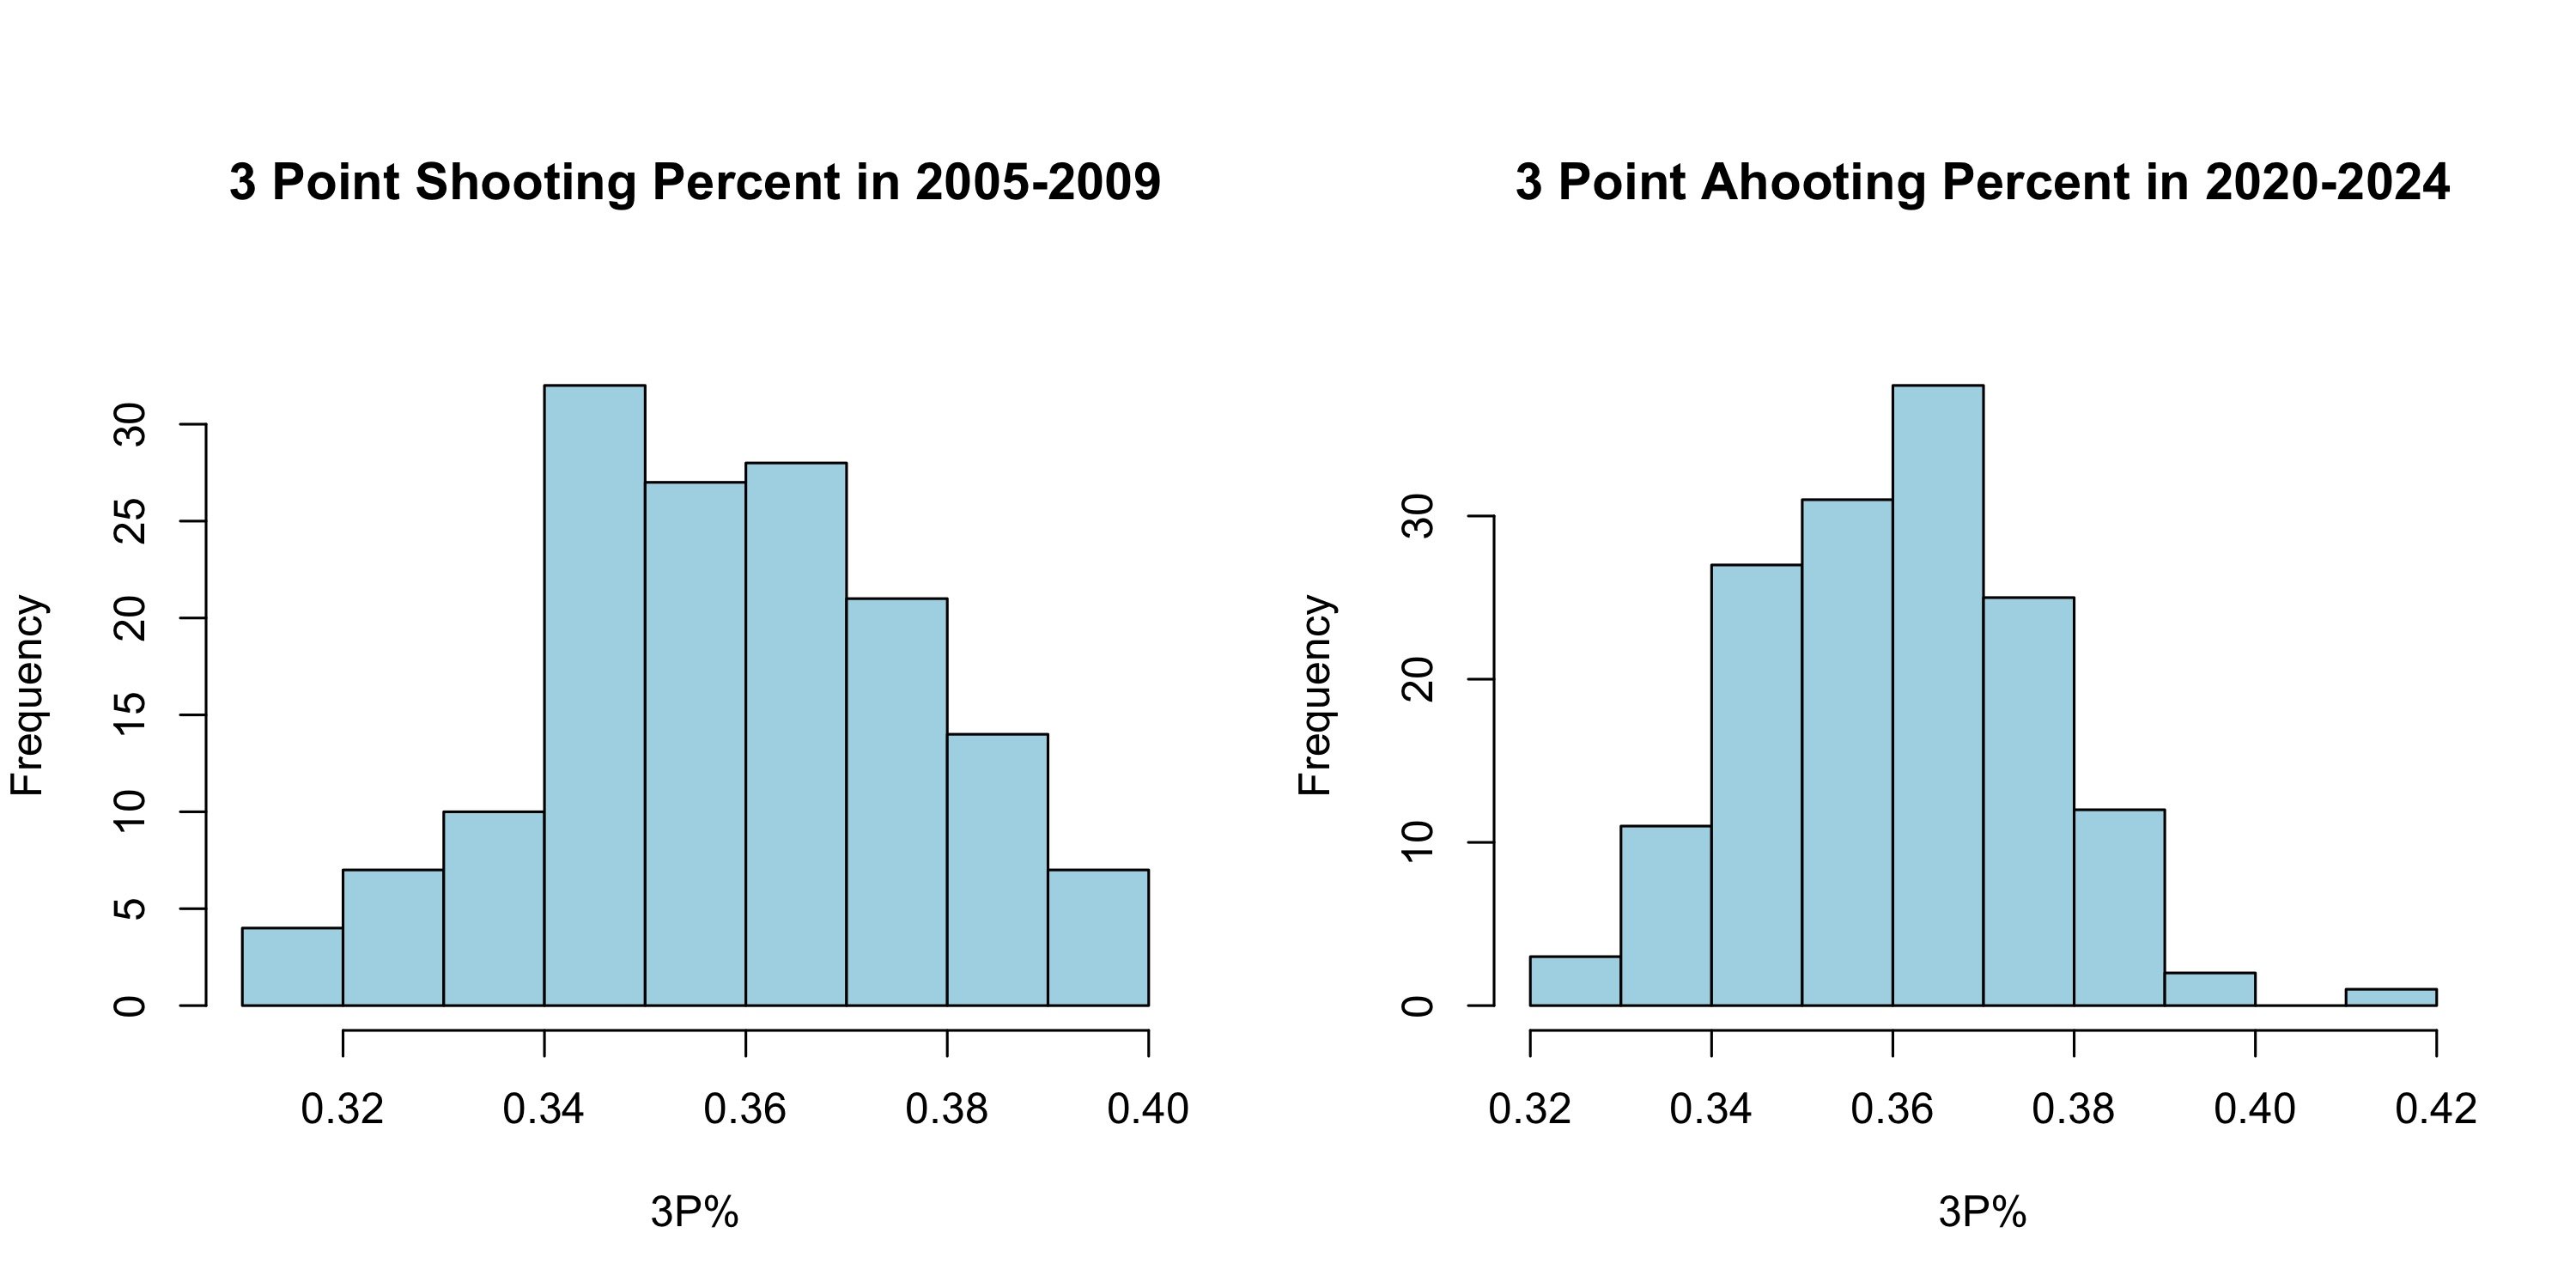
\includegraphics[width=0.9\textwidth]{figure/3P shooting percent.jpg}
    \caption{3 Point Shooting Percent in Two Different Period.}
    \label{fig:3P_shooting_percent}
\end{figure}

The second set of histograms(Figure \ref{fig:3P_attempt_rate}) displays the three-point attempt rate (3P\_ratio), defined as the proportion of a team's total field goal 
attempts that are three-pointers. We observe a substantial rightward shift over time: in the 2005–2009 period, teams clustered around a 
20\% attempt rate, whereas by 2020-2024, the distribution centers around 38-40\%. This sharp increase visually confirms the commonly 
cited notion that the NBA has entered a “small ball” era, characterized by greater reliance on perimeter shooting and faster-paced offenses.

\begin{figure}[htbp]
    \centering
    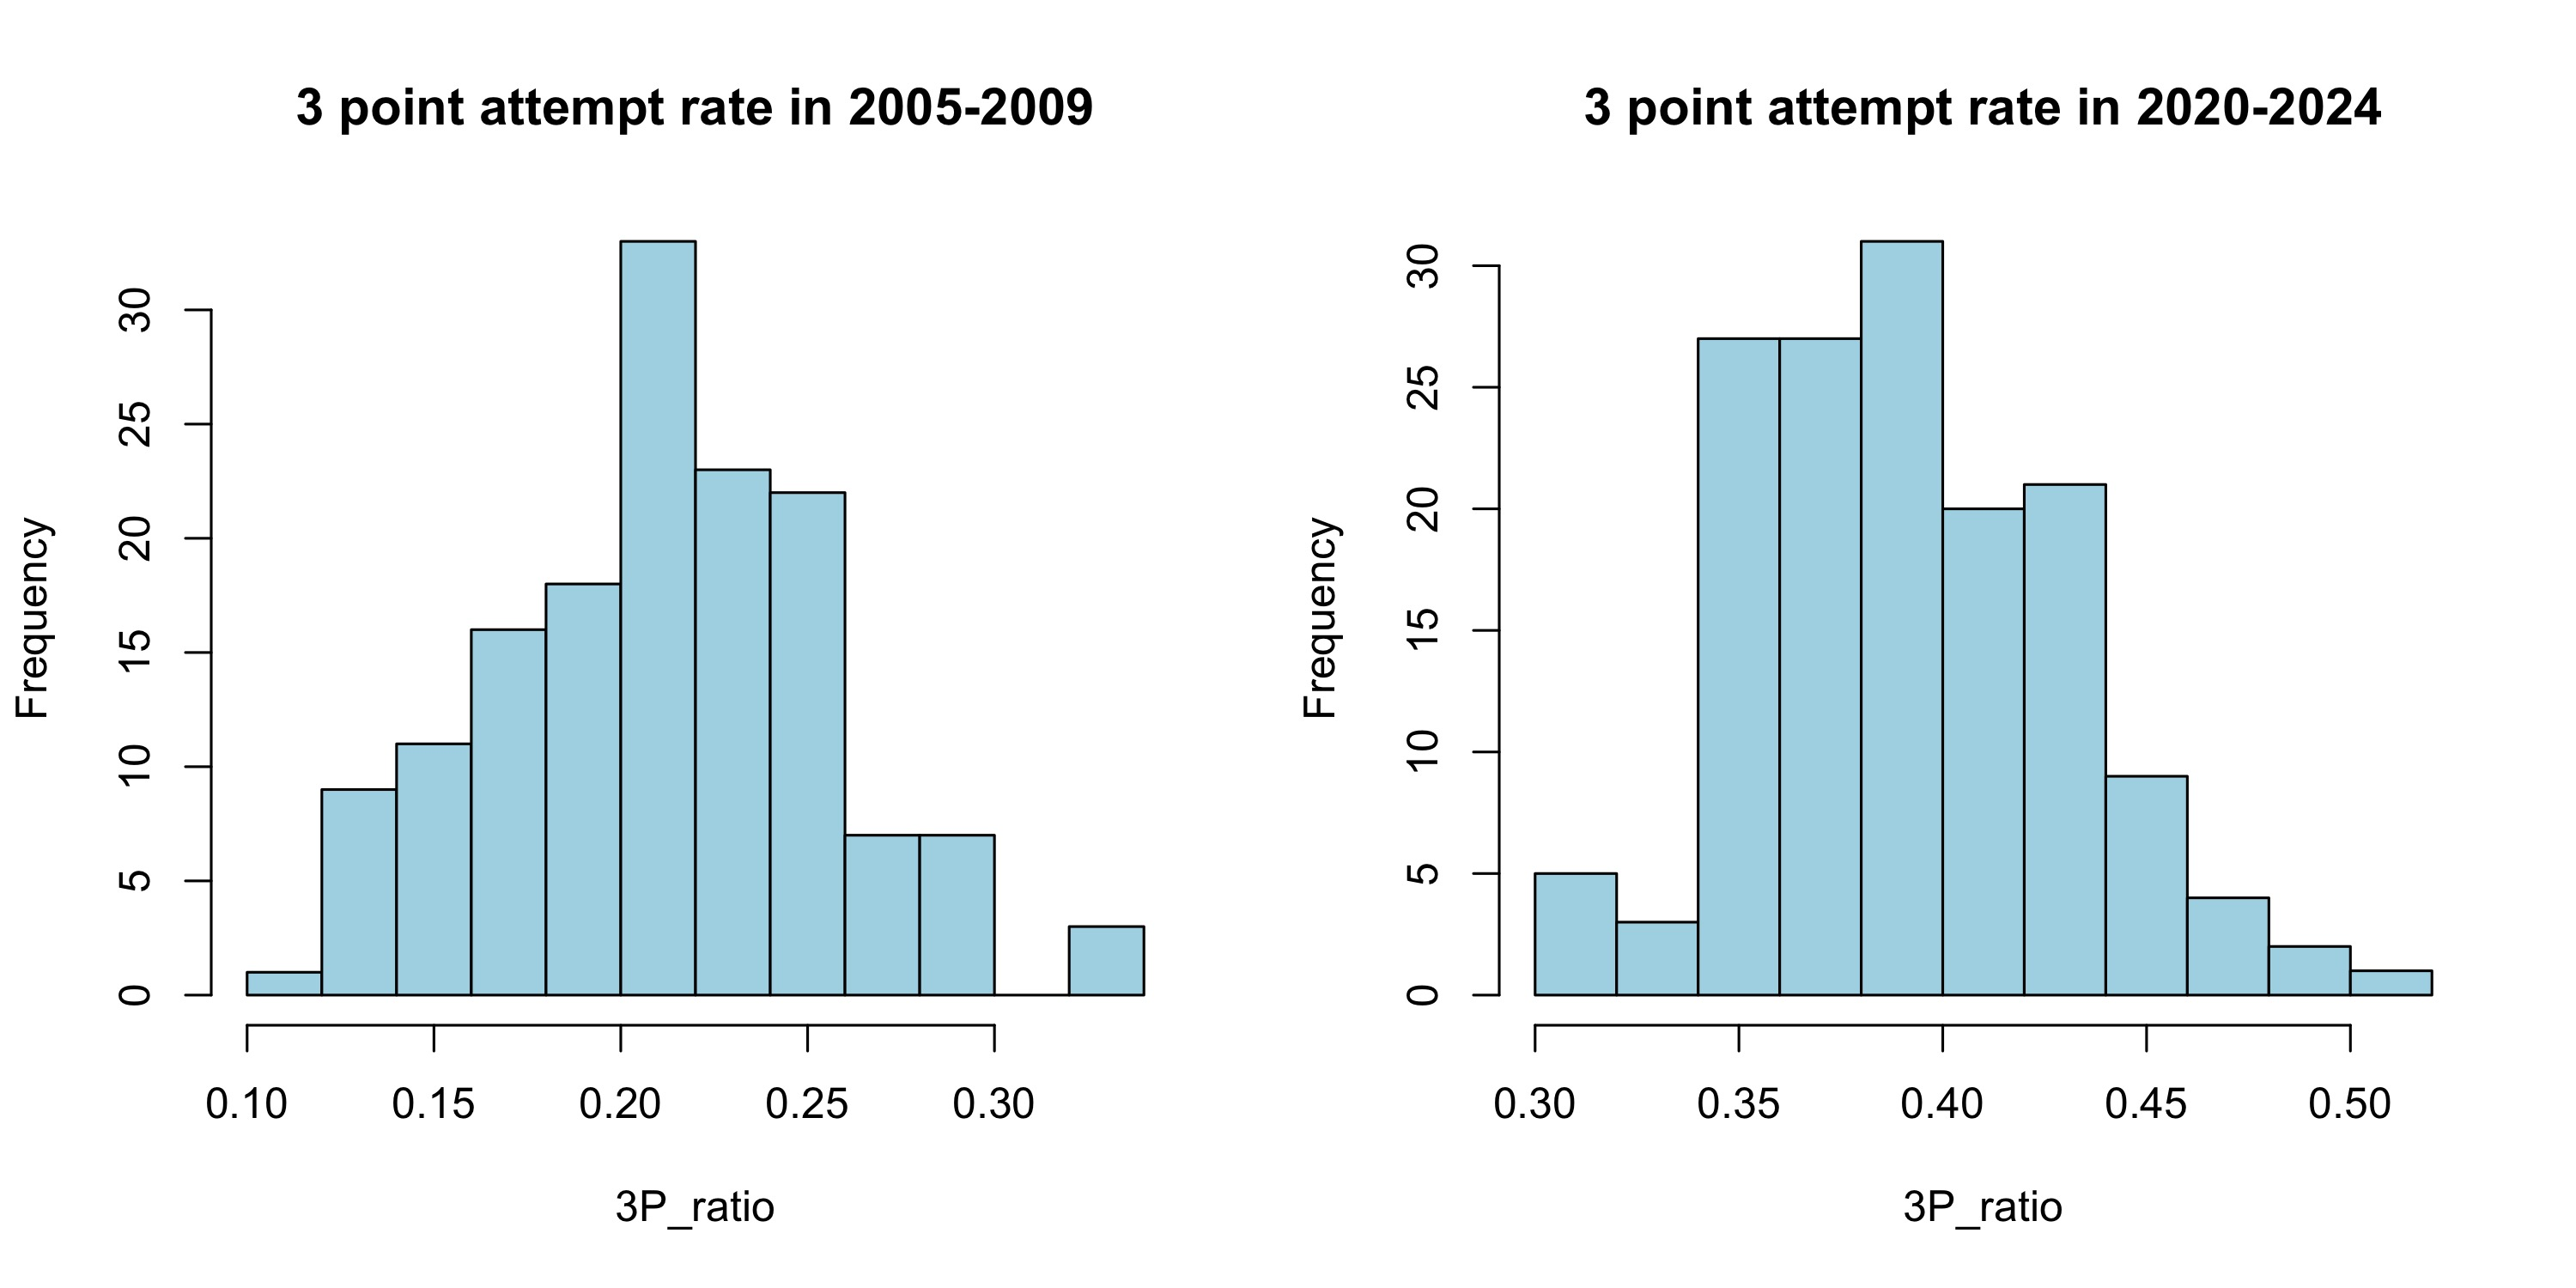
\includegraphics[width=0.9\textwidth]{figure/3 point attempt rate.jpg}
    \caption{3 Point Attempt Rate in Two Different Period.}
    \label{fig:3P_attempt_rate}
\end{figure}

Together, these visualizations provide structural evidence for a fundamental change in league-wide offensive strategy. 
The sharp increase in three-point attempt rates, coupled with stable or slightly improved three-point accuracy, sets the stage for our 
central analysis: evaluating whether and how the growing emphasis on three-point shooting translates into higher win rates in the modern NBA.


%---------------------------------------------------------------------------------
% Model
%---------------------------------------------------------------------------------

\section{Model}
\subsection{Model Specification}
To examine how the relationship between shooting efficiency and team success has evolved over time, we first fit a parsimonious linear 
regression model in each era, using team win rate (WinRate) as the dependent variable. The explanatory variables included three-point 
field goal percentage (3P\%), two-point field goal percentage (2P\%), and three-point attempt rate (3P\_ratio). 
\[
\text{WinRate} = \beta_0 + \beta_1 \times \text{3P\%} + \beta_2 \times \text{2P\%} + \beta_3 \times \text{3P\_ratio} + \epsilon
\]
This minimal specification 
allows us to isolate the marginal effects of shooting efficiency without the confounding influence of other team characteristics.

We separately fit the model to two distinct periods: the 2005--2009 seasons and the 2020--2024 seasons. The regression results reveal 
clear structural differences between eras.

In the 2005--2009 model, two-point field goal percentage (2P\%) is highly significant ($p \approx 3.11\times 10^{-08}$) and exhibits a strong positive 
relationship with win rate (coefficient = 3.7431). Three-point field goal percentage (3P\%) is statistically significant at the 1\% level 
($p \approx 0.0038$), which is just a 2 stars significant in R, and its impact (coefficient = 1.8842) is noticeably smaller than that of two-point 
efficiency. Three-point attempt rate (3P\_ratio) shows no statistical significance ($p \approx 0.301$). The detailed model summary is shown in 
Figire \ref{fig:model0_2005_2009} left.
\begin{figure}[htbp]
    \centering
    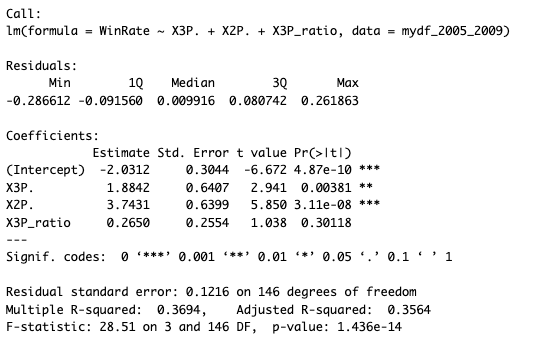
\includegraphics[width=0.45\textwidth]{figure/model0_2005_2009.png}
    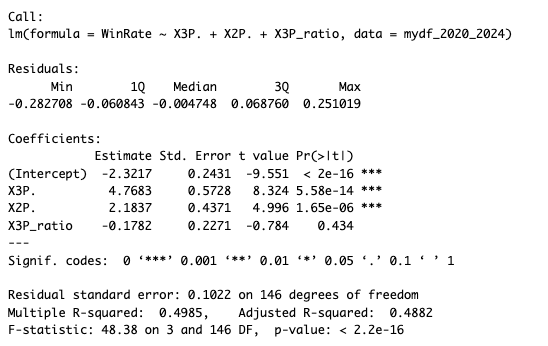
\includegraphics[width=0.45\textwidth]{figure/model0_2020_2024.png}
    \caption{model0 2005 2009.}
    \label{fig:model0_2005_2009}
\end{figure}

By contrast, in the 2020--2024 model, three-point field goal percentage (3P\%) becomes even more strongly significant ($p \approx 5.58 \times 10^{-14}$) 
and its marginal effect size increases substantially (coefficient = 4.7683). Meanwhile, the coefficient on two-point field goal percentage 
(2P\%) decreases to 2.1837, although it remains statistically significant. Again, three-point attempt rate (3P\_ratio) remains statistically 
insignificant. The detailed model summary is shown in Figire \ref{fig:model0_2005_2009} right.

These patterns suggest a fundamental shift:
\begin{itemize}
    \item In the earlier period, improving two-point shooting efficiency had a larger marginal benefit to team success than improving three-point 
    efficiency.
    \item In the modern period, improving three-point shooting efficiency has become more important than two-point efficiency, with its estimated 
    impact on win rate more than doubling the impact of two-point shooting.
\end{itemize}

This transition supports the hypothesis that the NBA has entered a ``three-point era,'' where teams' success increasingly depends on their ability to 
make three-point shots efficiently rather than solely relying on two-point scoring.

More than these two models, I also fit another two models in the periods 2010-2014 and 2015-2019. Using the data from these four models, I have create a 
table and a line chart. You can see the strong trend that 3P\% is more and more important with the time goes in the Table \ref{tab:coefficients_comparison} 
and the Figure \ref{fig:coefficients_comparison}.
\vspace{0.5cm}

\begin{table}[h]
\centering
\begin{tabular}{lcccc}
\hline
\textbf{Variable} & \textbf{2005-2009} & \textbf{2010-2014} & \textbf{2015-2019} & \textbf{2020-2024}  \\
\hline
3P\%(coefficient) & 1.8842 & 2.6011 & 3.8326  & 4.7683  \\
2P\%(coefficient) & 3.7431 & 4.0901 & 3.1201 & 2.1837  \\
3P\%(significance) & 0.00381 & $4.09 \times 10^{-6}$ & $1.13 \times 10^{-9}$ & $5.58 \times 10^{-14}$  \\
2P\%(significance) & $3.11 \times 10^{-8}$  & $1.64 \times 10^{-12}$ & $1.51 \times 10^{-8}$ & $1.65 \times 10^{-6}$  \\
3P\_ratio(significance) & 0.30118 (n.s.) & 0.191 (n.s.) & 0.0966 (n.s.) & 0.434 (n.s.)\\
\hline
\end{tabular}
\caption{Comparison of Marginal Effects Between Periods}
\label{tab:coefficients_comparison}
\end{table}
\begin{figure}[htbp]
    \centering
    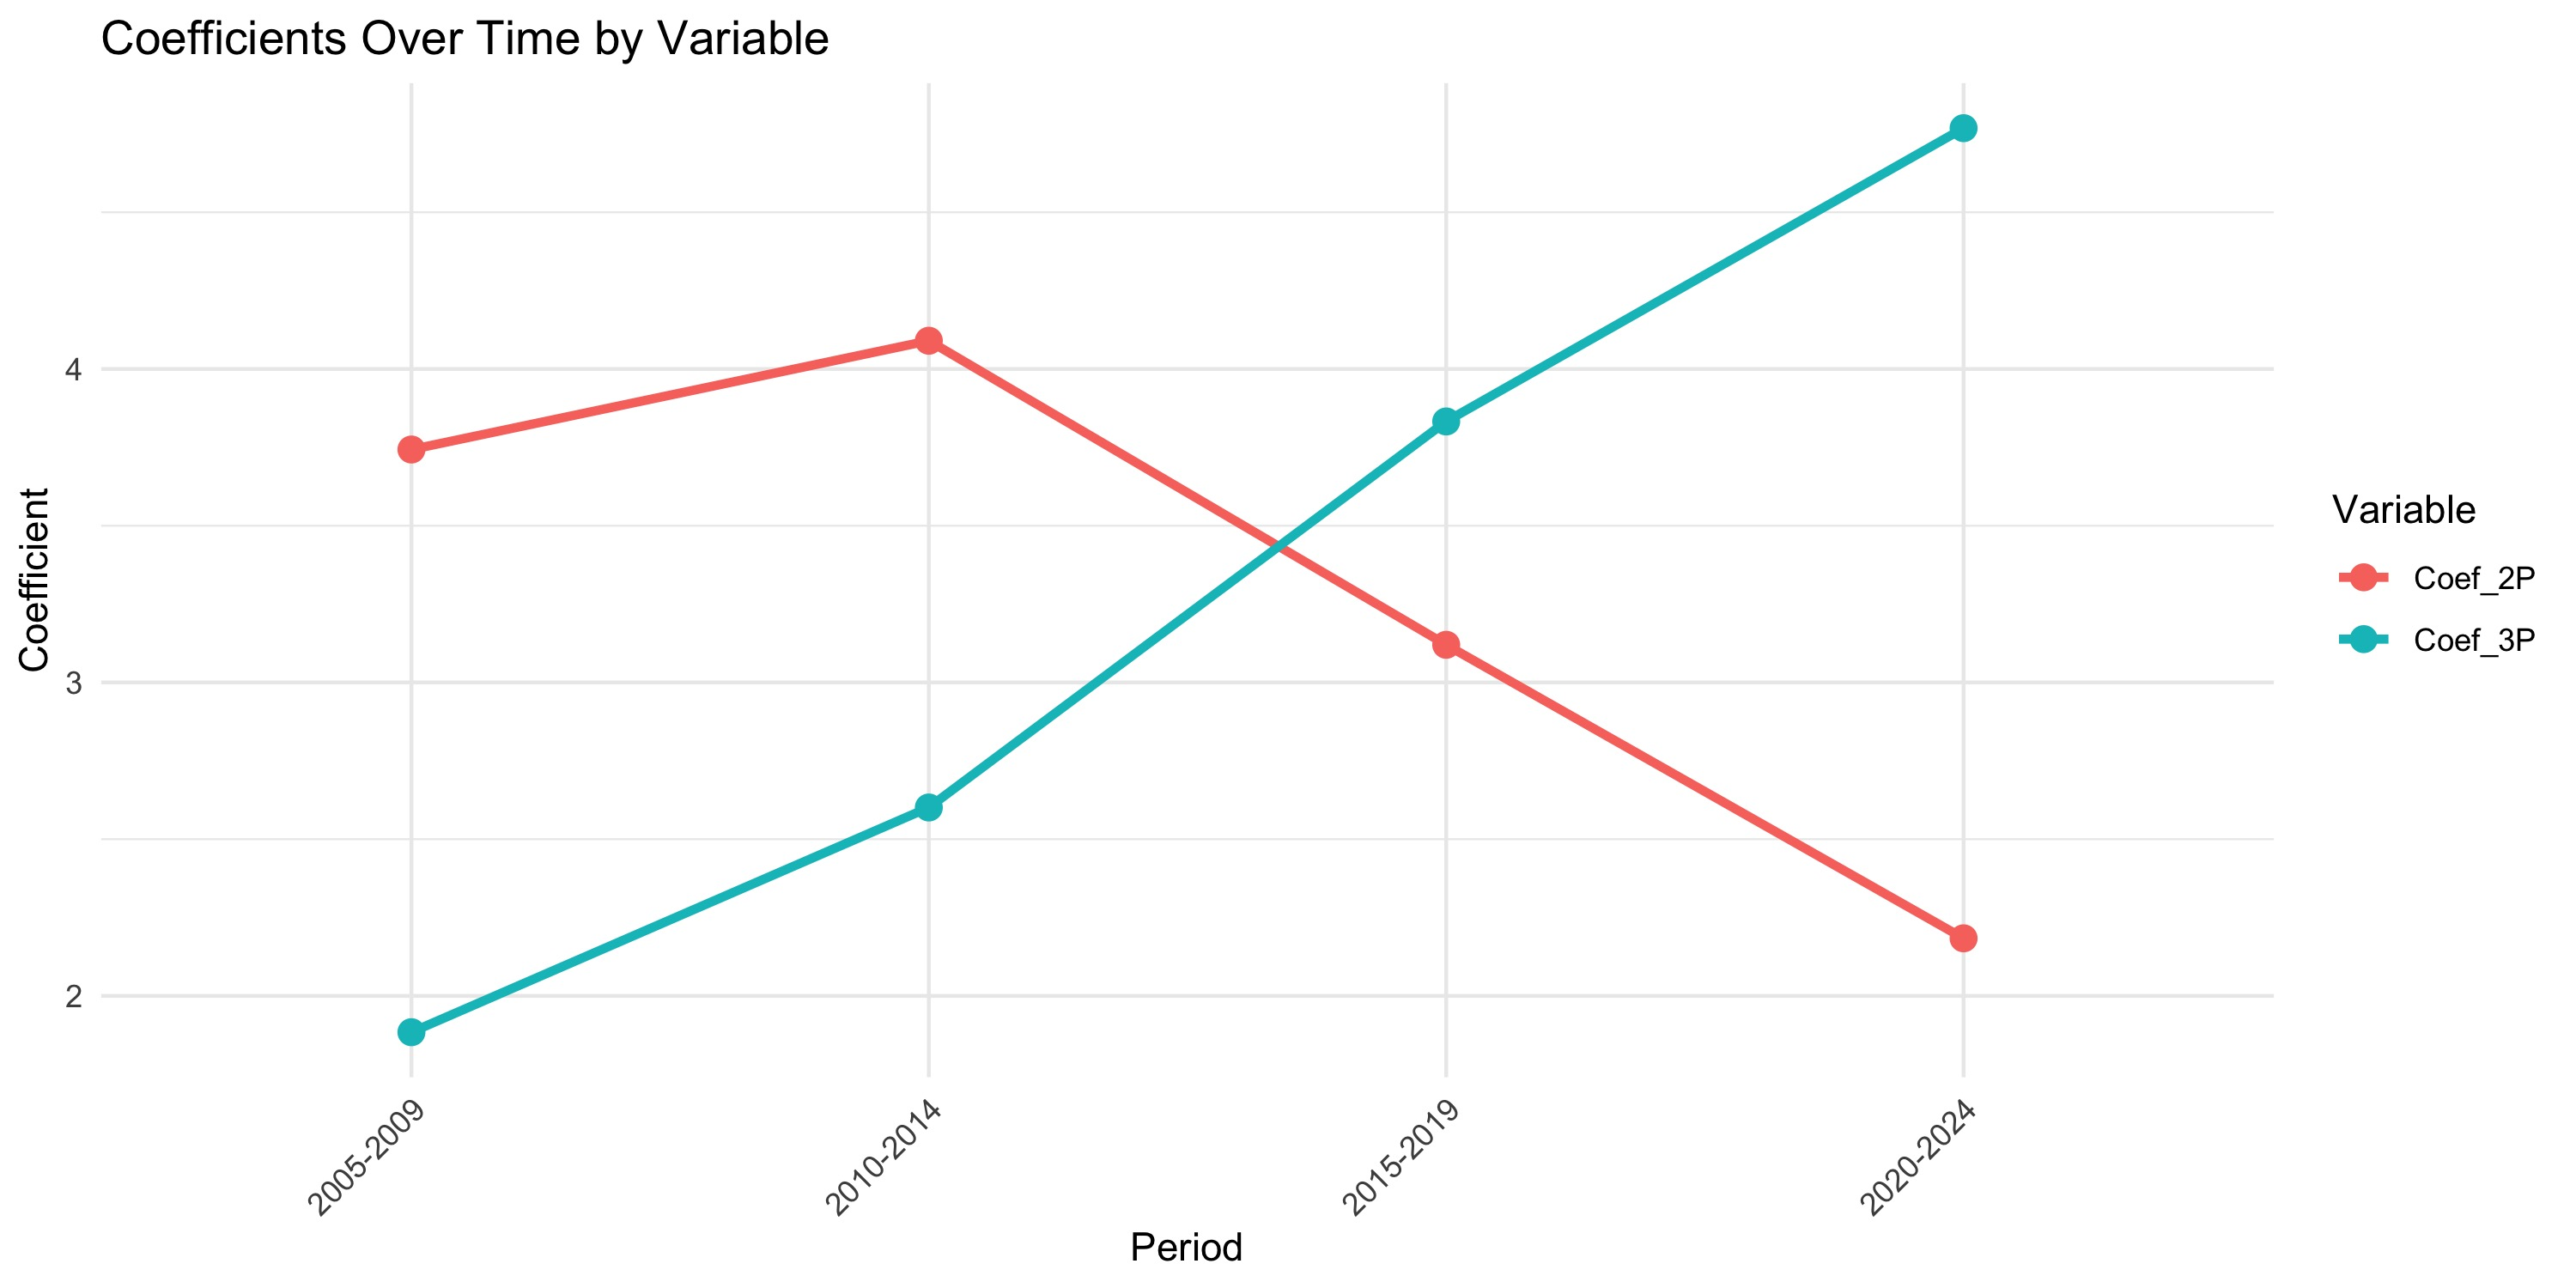
\includegraphics[width=0.45\textwidth]{figure/Coefficients Over Time by Variable.jpg}
    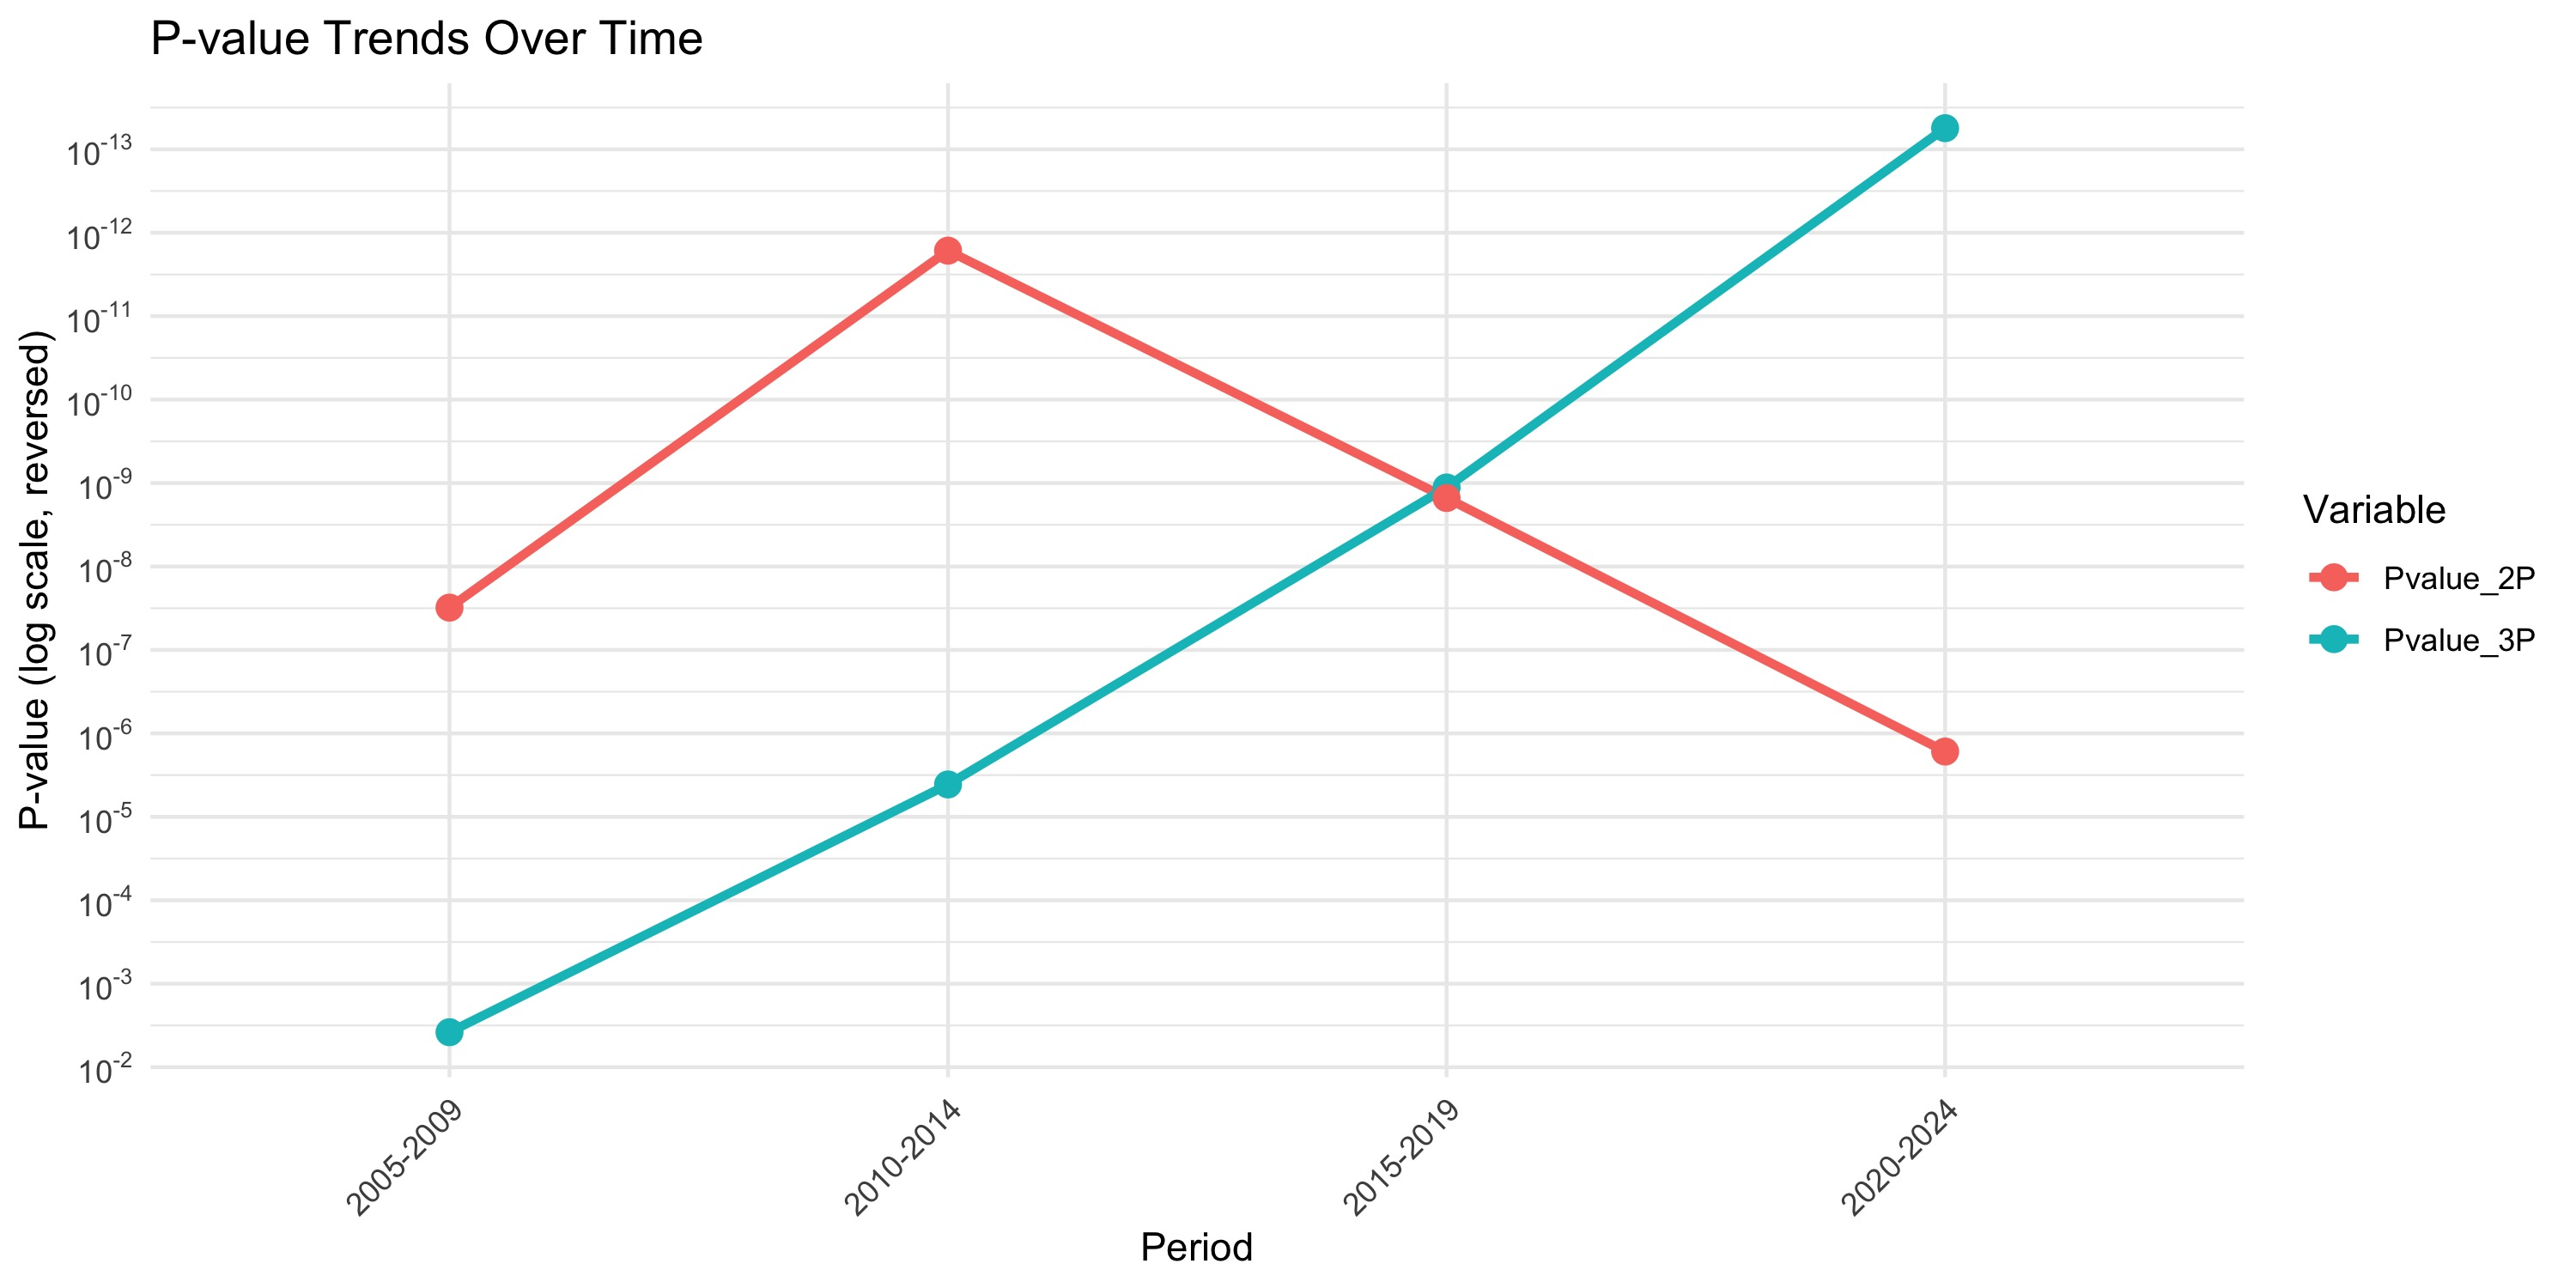
\includegraphics[width=0.45\textwidth]{figure/P-value Trends Over Time.jpg}
    \caption{Comparison of Marginal Effects Between Periods.}
    \label{fig:coefficients_comparison}
\end{figure}

\subsection{Model Diagnostic}



%----------------------------------------------------------------------------------------
% Conclusion
%----------------------------------------------------------------------------------------

\section{Conclusion}

%----------------------------------------------------------------------------------------
% Conclusion
%----------------------------------------------------------------------------------------

\newpage % Includes a new page
\pagenumbering{roman} % Changes page numbering to roman page numbers
%\bibliography{literature}

\bibliography{literature.bib} % Add the filename of your bibliography
\bibliographystyle{apsr} % Defines your bibliography style

%----------------------------------------------------------------------------------------
% Conclusion
%----------------------------------------------------------------------------------------

\newpage
\pagenumbering{roman} % Changes page numbering to roman page numbers

\section*{Appendix}

% For citing, please see this sheet: http://merkel.texture.rocks/Latex/natbib.php

% %----------------------------------------------------------------------------------------
% % Appendix
% %----------------------------------------------------------------------------------------
% \newpage % Includes a new page
% \section*{Appendix} % Stars disable section numbers
% % \appendix % Uncomment if you want to add an "automatic" appendix
% \pagenumbering{Roman} % Changes page numbering to Roman page numbers

% \blindtext % Adds some blind text

% %----------------------------------------------------------------------------------------
% % Declaration
% %----------------------------------------------------------------------------------------
% \newpage % Includes a page break
% \thispagestyle{empty} % Leaves the page style empty (no page number, no header, no footer)
% \section*{Statutory Declaration} % Stars disable section numbers

% \begin{otherlanguage}{german}
% Hiermit versichere ich, dass diese Arbeit von mir pers\"{o}nlich verfasst ist und dass ich keinerlei fremde Hilfe in Anspruch genommen habe. Ebenso versichere ich, dass diese Arbeit oder Teile daraus weder von mir selbst noch von anderen als Leistungsnachweise andernorts eingereicht wurden. W\"{o}rtliche oder sinngem\"{a}{\ss}e \"{U}bernahmen aus anderen Schriften und Ver\"{o}ffentlichungen in gedruckter oder elektronischer Form sind gekennzeichnet. S\"{a}mtliche Sekund\"{a}rliteratur und sonstige Quellen sind nachgewiesen und in der Bibliographie aufgef\"{u}hrt. Das Gleiche gilt f\"{u}r graphische Darstellungen und Bilder sowie f\"{u}r alle Internet-Quellen. Ich bin ferner damit einverstanden, dass meine Arbeit zum Zwecke eines Plagiatsabgleichs in elektronischer Form anonymisiert versendet und gespeichert werden kann. Mir ist bekannt, dass von der Korrektur der Arbeit abgesehen und die Pr\"{u}fungsleistung mit nicht ausreichend bewertet werden kann, wenn die Erkl\"{a}rung nicht erteilt wird.
% \end{otherlanguage}

% \vspace*{1in} % Adds extra space between two paragraphs

% \noindent I hereby declare that the paper presented is my own work and that I have not called upon the help of a third party. In addition, I affirm that neither I nor anybody else has submitted this paper or parts of it to obtain credits elsewhere before. I have clearly marked and acknowledged all quotations or references that have been taken from the works of others. All secondary literature and other sources are marked and listed in the bibliography. The same applies to all charts, diagrams and illustrations as well as to all Internet resources. Moreover, I consent to my paper being electronically stored and sent anonymously in order to be checked for plagiarism. I am aware that the paper cannot be evaluated and may be graded ``failed'' (``nicht ausreichend'') if the declaration is not made.\\

% %\vspace*{1in} % Adds extra space

% % Add field for signature, date, and place
% \hfill \signature{} 


% %---------------------------------------------------------------------------------

\end{document}
